\documentclass[tikz]{standalone}
\usepackage{bm}
\usepackage{stix}

\usetikzlibrary{calc}

\definecolor{mplblue}{HTML}{1f77b4}
\definecolor{mplmagenta}{HTML}{e377c2}

\tikzstyle{site}=[rounded corners, minimum size=1cm, inner sep=0, draw=mplblue!80!black, fill=mplblue!20!white]
\tikzstyle{kron}=[circle, draw, fill, minimum size=0.1cm, inner sep=0]

\begin{document}
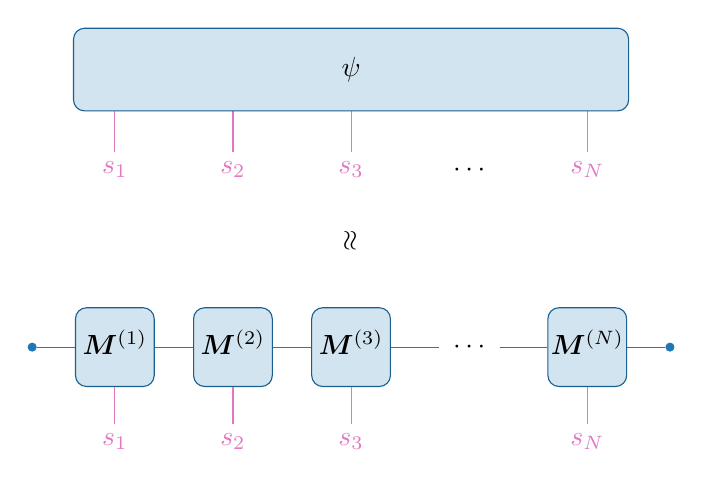
\begin{tikzpicture}[x=1.5cm, y=1.5cm]

\node [site] (M1) at (0, 0) {$\strut \bm{M}^{(1)}$};
\node [site] (M2) at (1, 0) {$\strut \bm{M}^{(2)}$};
\node [site] (M3) at (2, 0) {$\strut \bm{M}^{(3)}$};
\node        (Me) at (3, 0) {$\strut \cdots {}$};
\node [site] (MN) at (4, 0) {$\strut \bm{M}^{(N)}$};

\node [kron, mplblue] (l) at (-0.7, 0) {};
\node [kron, mplblue] (r) at ( 4.7, 0) {};

\node [text=mplmagenta] (s1) at (0, -0.8) {$s_1$};
\node [text=mplmagenta] (s2) at (1, -0.8) {$s_2$};
\node [text=mplmagenta] (s3) at (2, -0.8) {$s_3$};
\node [text=mplmagenta] (sN) at (4, -0.8) {$s_N$};

\draw [mplblue] (M1) -- (M2);
\draw [mplblue] (M2) -- (M3);
\draw [mplblue] (M3) -- (Me);
\draw [mplblue] (Me) -- (MN);

\draw [mplblue] (l) -- (M1);
\draw [mplblue] (MN) -- (r);

\draw [mplmagenta] (M1) -- (s1);
\draw [mplmagenta] (M2) -- (s2);
\draw [mplmagenta] (M3) -- (s3);
\draw [mplmagenta] (MN) -- (sN);

\node [text=mplmagenta] (s1) at (0, 1.5) {$s_1$};
\node [text=mplmagenta] (s2) at (1, 1.5) {$s_2$};
\node [text=mplmagenta] (s3) at (2, 1.5) {$s_3$};
\node                   (se) at (3, 1.5) {$\cdots$};
\node [text=mplmagenta] (sN) at (4, 1.5) {$s_N$};

\draw [mplmagenta] (0, 2) -- (s1);
\draw [mplmagenta] (1, 2) -- (s2);
\draw [mplmagenta] (2, 2) -- (s3);
\draw [mplmagenta] (4, 2) -- (sN);

\draw [rounded corners, draw=mplblue!80!black, fill=mplblue!20!white] (-0.35, 2) rectangle (4.35, 2.7);

\node at (2, 2.35) {$\strut \psi$};
\node [rotate=90] at (2, 0.9) {$\approx$};

\end{tikzpicture}
\end{document}
